\documentclass{article}

\usepackage{graphicx}
\usepackage{subcaption}
\usepackage[margin=1in]{geometry}			%margins
\usepackage{indentfirst}					%indentation
\usepackage{listings}						%code
\usepackage{amsmath}

\setlength{\intextsep}{15pt plus 1.0pt minus 2.0pt}		%figure spacing inside text

\begin{document}

\title{STAT 239 Homework 4}
\author{Tarek Tohme}
\date{June 7th, 2018}
\maketitle

\section*{Data Analysis 1}

\paragraph{}
% Figure 1: plots
\begin{figure}[h]				%placement (here)
	\centering
	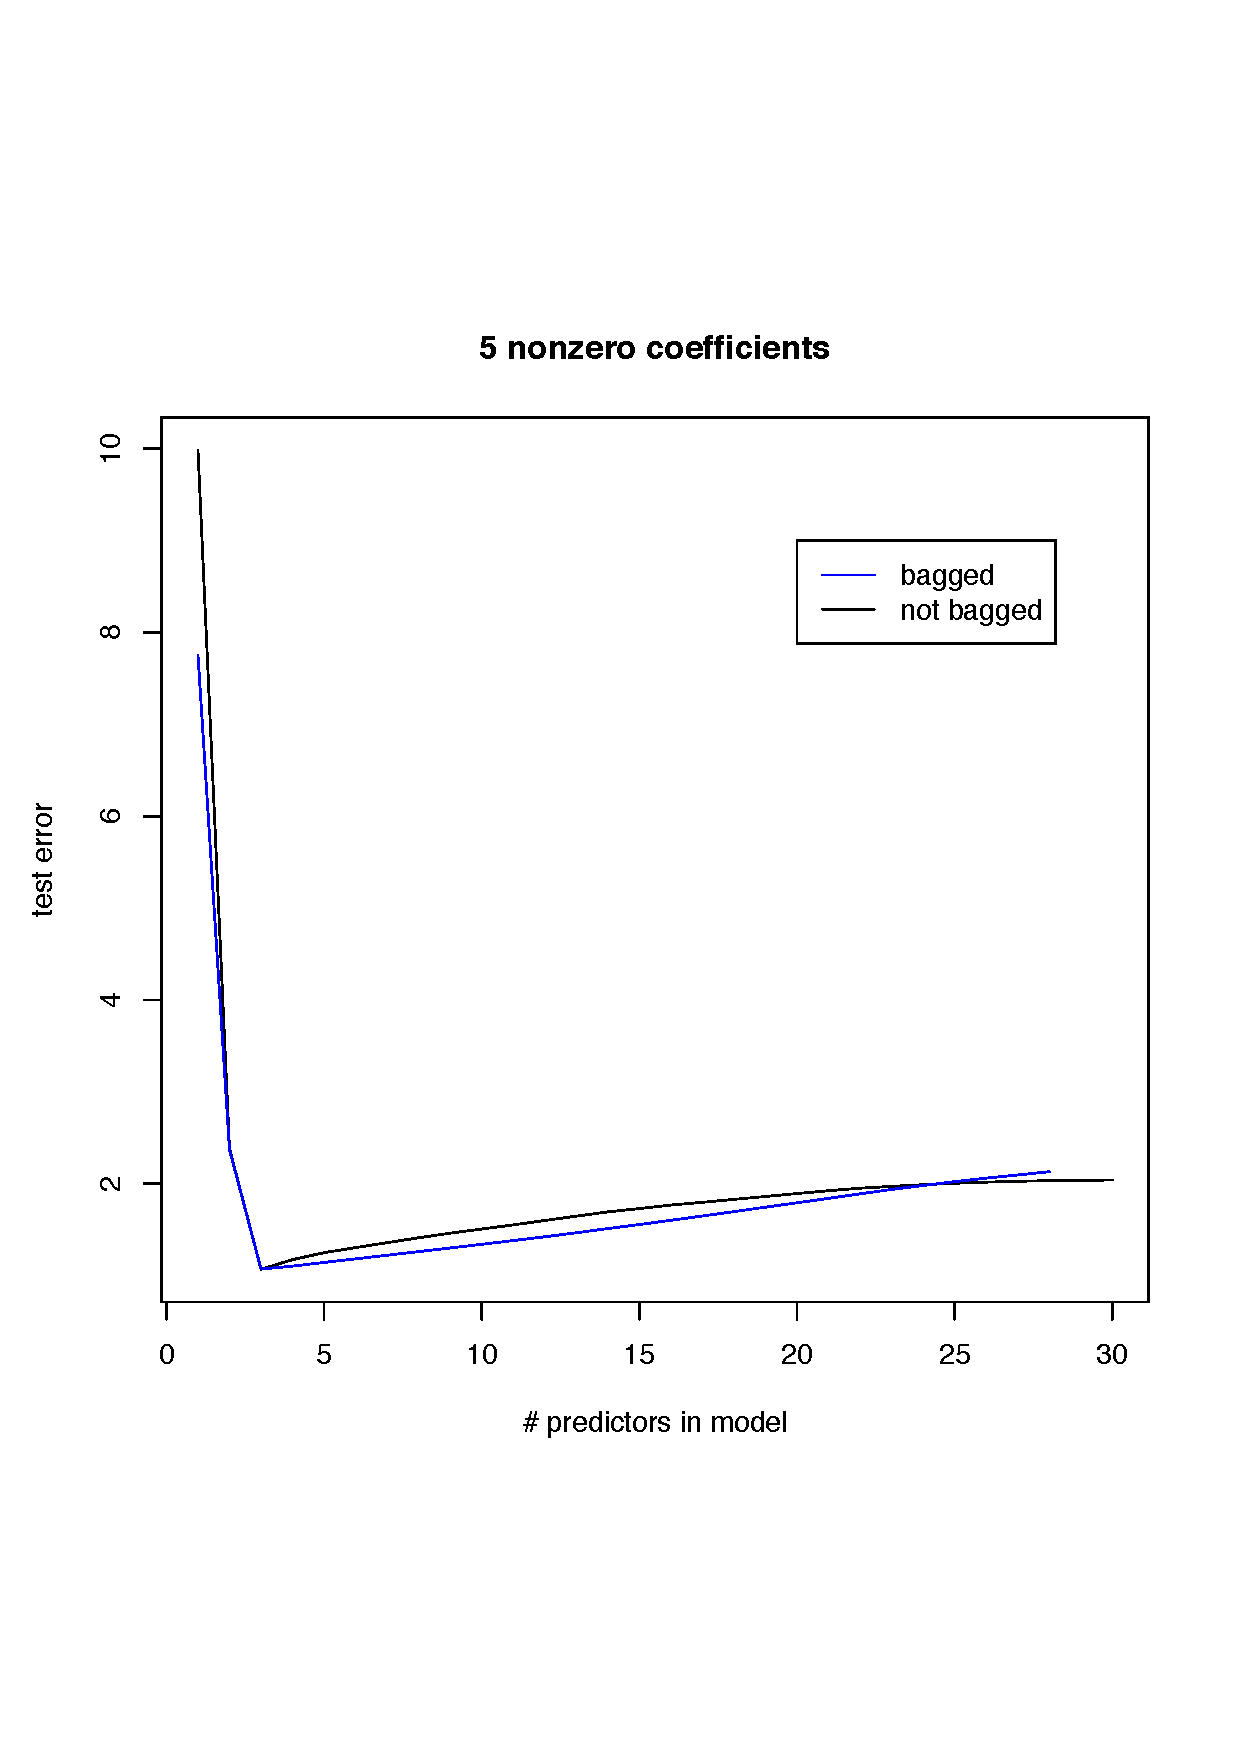
\includegraphics[width=8.2cm]{DA1/5.pdf}
	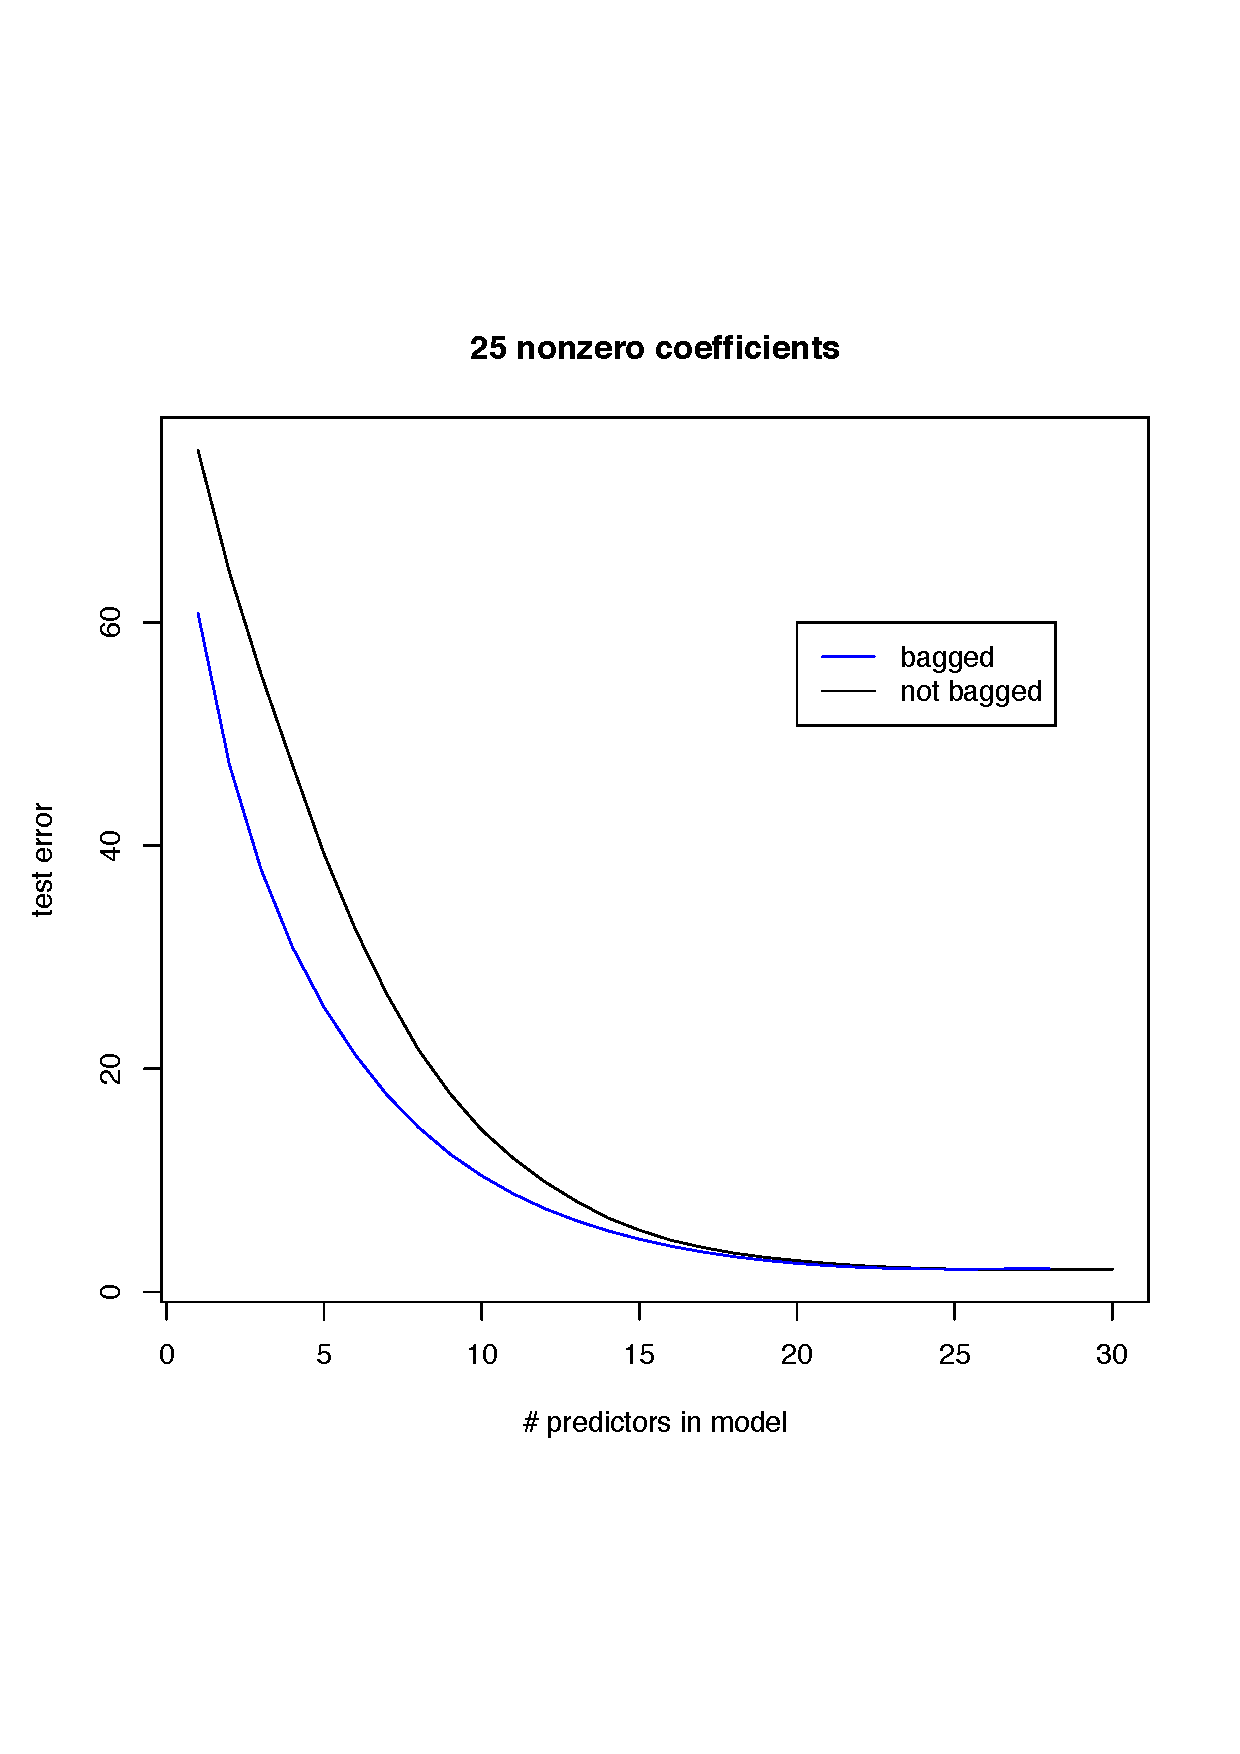
\includegraphics[width=8.2cm]{DA1/25.pdf}
	\caption{}
\end{figure}

The minimum error is achieved at the same point for both plots.
The bagged prediction error is lower for models with few predictors in both situations. As the number of predictors in the model increases, the difference between the bagged error and the regular error shrinks until the bagged error becomes greater. This will be explained in the context of the decomposition of the error, reproduced from the notes4 file below,

\begin{equation*}
Error = E(\epsilon^2) + E_X\left[\left(F(X) - E_T\hat{F}(X,T)\right)^2\right] + E_{X,T}\left[\left(\hat{F}(X, T) - E_T\hat{F}(X,T)\right)^2\right]
\end{equation*}

Since we are averaging over 300 simulated samples for both the bagged and non-bagged models, the irreducible error is shrunken by the same amount in both. Therefore it cannot be causing a difference in the prediction error. The bias term also cannot be causing a difference in the error between both models since, as outlined in the notes, the limit of the bootstrapped model approximates the expected value of the learner over the training data,

\begin{equation*}
E_T(h(T)) \approx \operatorname*{lim}_{B \to \infty} \frac{1}{B}\sum_{b=1}^Bh(T_b)
\end{equation*} 

which has the same bias as the learner itself. Thus, the difference is due to the variance term. The bagged model's error is reduced most when the bootstrapped learners are least correlated among each other. This happens when there are fewer coefficients in the model being fitted. In a model with a smaller number of coefficients, each coefficient has to account for greater variability in the data. This results in less correlation between coefficients of different learners. An extreme example would be a model with a single nonzero coefficient, fitted on a dataset with many principal components. Such a model would have to account for all the variability of the data with a single predictor, and thus the correlation between two such bootstrapped learners would be directly related to the correlation of the data samples, and so would be very small since the samples are supposedly random. This is the situation where bagging is beneficial, since it reduces this variability in the predictor. In the other extreme, if there were too many predictors in the model, each one would capture a specific part of the variability of the data, and hence would vary less across samples, resulting in a higher correlation among the learners fitted on these samples. If there are more coefficients in the model than needed to capture all the variability in the data (as it happens in the figure on the left after 25 predictors) then eventually the added variance of the useless predictors that capture only noise outweighs the reduction in variance granted by bagging.

\section*{Data Analysis 2}


\end{document}


